\documentclass[11pt,a4paper,oneside]{report}             % Single-side

%\PassOptionsToPackage{chapternumber=Huordinal}{magyar.ldf}
\usepackage{t1enc}
\usepackage[utf8]{inputenc}
\usepackage{amsmath}
\usepackage{amssymb}
\usepackage{enumerate}
\usepackage[amsmath,thmmarks]{ntheorem}
\usepackage{graphics}
\usepackage{epsfig}
\usepackage{listings}
\usepackage{color}
%\usepackage{fancyhdr}
\usepackage{lastpage}
\usepackage{anysize}
\usepackage[english]{babel}
\usepackage{sectsty}
\usepackage{setspace}  % Ettol a tablazatok, abrak, labjegyzetek maradnak 1-es sorkozzel!
\usepackage[hang]{caption}
\usepackage{hyperref}
\usepackage[final]{pdfpages}
%\usepackage{minted}
\usepackage{lscape}
\usepackage{float}


%--------------------------------------------------------------------------------------
% Main variables
%--------------------------------------------------------------------------------------
\newcommand{\vikszerzo}{Dávid Danyi}
\newcommand{\vikkonzulens}{Viktor Kovács}
\newcommand{\vikcim}{Marker Based Localisation and Pose Estimation Using Image Processing}
\newcommand{\viktanszek}{Department of Automation and Applied Informatics}
\newcommand{\vikdoktipus}{Thesis}
\newcommand{\vikdepartmentr}{Dávid Danyi}

%--------------------------------------------------------------------------------------
% Page layout setup
%--------------------------------------------------------------------------------------
% we need to redefine the pagestyle plain
% another possibility is to use the body of this command without \fancypagestyle
% and use \pagestyle{fancy} but in that case the special pages
% (like the ToC, the References, and the Chapter pages)remain in plane style

\pagestyle{plain}
\setlength{\parindent}{0pt} % áttekinthetőbb, angol nyelvű dokumentumokban jellemző
\setlength{\parskip}{8pt plus 3pt minus 3pt} % áttekinthetőbb, angol nyelvű dokumentumokban jellemző
%\setlength{\parindent}{12pt} % magyar nyelvű dokumentumokban jellemző
%\setlength{\parskip}{0pt}    % magyar nyelvű dokumentumokban jellemző

\marginsize{35mm}{25mm}{15mm}{15mm} % anysize package
\setcounter{secnumdepth}{0}
\sectionfont{\large\upshape\bfseries}
\setcounter{secnumdepth}{2}
\singlespacing
\frenchspacing

%--------------------------------------------------------------------------------------
%	Setup hyperref package
%--------------------------------------------------------------------------------------
\hypersetup{
    bookmarks=true,            % show bookmarks bar?
    unicode=false,             % non-Latin characters in Acrobat’s bookmarks
    pdftitle={\vikcim},        % title
    pdfauthor={\vikszerzo},    % author
    pdfsubject={\vikdoktipus}, % subject of the document
    pdfcreator={\vikszerzo},   % creator of the document
    pdfproducer={Producer},    % producer of the document
    pdfkeywords={keywords},    % list of keywords
    pdfnewwindow=true,         % links in new window
    colorlinks=true,           % false: boxed links; true: colored links
    linkcolor=black,           % color of internal links
    citecolor=black,           % color of links to bibliography
    filecolor=black,           % color of file links
    urlcolor=black             % color of external links
}

%--------------------------------------------------------------------------------------
% Set up listings
%--------------------------------------------------------------------------------------
\lstset{
	basicstyle=\scriptsize\ttfamily, % print whole listing small
	keywordstyle=\color{black}\bfseries\underbar, % underlined bold black keywords
	identifierstyle=, 					% nothing happens
	commentstyle=\color{white}, % white comments
	stringstyle=\scriptsize\sffamily, 			% typewriter type for strings
	showstringspaces=false,     % no special string spaces
	aboveskip=3pt,
	belowskip=3pt,
	columns=fixed,
	backgroundcolor=\color{lightgray},
} 		
\def\lstlistingname{listing}

%--------------------------------------------------------------------------------------
% Set up minted
%--------------------------------------------------------------------------------------	
%\definecolor{bg}{rgb}{0.95,0.95,0.95}
%\usemintedstyle{emacs}

%--------------------------------------------------------------------------------------
%	Some new commands and declarations
%--------------------------------------------------------------------------------------
\newcommand{\code}[1]{{\upshape\ttfamily\scriptsize\indent #1}}

% define references
\newcommand{\figref}[1]{\ref{fig:#1}.}
\renewcommand{\eqref}[1]{(\ref{eq:#1})}
\newcommand{\listref}[1]{\ref{listing:#1}.}
\newcommand{\sectref}[1]{\ref{sect:#1}}
\newcommand{\tabref}[1]{\ref{tab:#1}.}

\DeclareMathOperator*{\argmax}{arg\,max}
%\DeclareMathOperator*[1]{\floor}{arg\,max}
\DeclareMathOperator{\sign}{sgn}
\DeclareMathOperator{\rot}{rot}
\definecolor{lightgray}{rgb}{0.95,0.95,0.95}

\author{\vikszerzo}
\title{\viktitle}
\includeonly{
	titlepage,%
	declaration,%
	abstract,%
	abbreviations,%
	introduction,%
	marker,%
	markerRec,%
	%chapter3,%
	conclusion, %
	appendices,%
}

%--------------------------------------------------------------------------------------
%	Setup captions
%--------------------------------------------------------------------------------------
\captionsetup[figure]{
%labelsep=none,
%font={footnotesize,it},
%justification=justified,
width=.75\textwidth,
aboveskip=10pt}

\renewcommand{\captionlabelfont}{\small\bf}
\renewcommand{\captionfont}{\footnotesize\it}

%--------------------------------------------------------------------------------------
% Table of contents and the main text
%--------------------------------------------------------------------------------------
\begin{document}

\includepdf{feladatkiiras.pdf}
\pagenumbering{arabic}
\onehalfspacing
%--------------------------------------------------------------------------------------
%	The title page
%--------------------------------------------------------------------------------------
\begin{titlepage}
\begin{center}

\includegraphics[width=60mm,keepaspectratio]{figures/BMElogo.png}\\
\vspace{0.3cm}
\textbf{Budapest University of Technology and Economics}\\
\textmd{Faculty of Electrical Engineering and Informatics}\\
\textmd{\viktanszek}\\[5cm]

\vspace{0.4cm}
{\huge \bfseries \vikcim}\\[0.8cm]
\vspace{0.5cm}
\textsc{\Large \vikdoktipus}\\[4cm]

\begin{tabular}{cc}
 \makebox[7cm]{\emph{Author}} & \makebox[7cm]{\emph{Consultant}} \\
 \makebox[7cm]{\vikszerzo} & \makebox[7cm]{\vikkonzulens}
\end{tabular}

\vfill
{\large \today}
\end{center}
\end{titlepage}
\tableofcontents\vfill
%--------------------------------------------------------------------------------------
% Nyilatkozat
%--------------------------------------------------------------------------------------
\begin{center}
\large
\textbf{HALLGATÓI NYILATKOZAT}\\
\end{center}

Alulírott \emph{\vikszerzo}, szigorló hallgató kijelentem, hogy ezt a szakdolgozatot meg nem engedett segítség nélkül, saját magam készítettem, csak a megadott forrásokat (szakirodalom, eszközök stb.) használtam fel. Minden olyan részt, melyet szó szerint, vagy azonos értelemben, de átfogalmazva más forrásból átvettem, egyértelmûen, a forrás megadásával megjelöltem.

Hozzájárulok, hogy a jelen munkám alapadatait (szerzõ(k), cím, angol és magyar nyelvû tartalmi kivonat, készítés éve, konzulens(ek) neve) a BME VIK nyilvánosan hozzáférhetõ elektronikus formában, a munka teljes szövegét pedig az egyetem belsõ hálózatán keresztül (vagy autentikált felhasználók számára) közzétegye. Kijelentem, hogy a benyújtott munka és annak elektronikus verziója megegyezik. Dékáni engedéllyel titkosított diplomatervek esetén a dolgozat szövege csak 3 év eltelte után válik hozzáférhetõvé.

\begin{flushleft}
\vspace*{1cm}
Budapest, \today
\end{flushleft}

\begin{flushright}
 \vspace*{1cm}
 \makebox[7cm]{\rule{6cm}{.4pt}}\\
 \makebox[7cm]{\emph{\vikszerzo}}\\
 \makebox[7cm]{hallgató}
\end{flushright}
\thispagestyle{empty}

\vfill
\clearpage
\thispagestyle{empty} % an empty page


%----------------------------------------------------------------------------
% Abstract in hungarian
%----------------------------------------------------------------------------
\chapter*{Kivonat}\addcontentsline{toc}{chapter}{Kivonat}
A képfeldolgozás nem újkeletű tudományterület, már évtizedek óta folynak kutatások ezen a téren.
Sok, ma is használt algoritmust az 1960-as években fejlesztettek ki.
Akkoriban főleg a tudósok körében használt, drága eszköznek számított a számítógépes képfeldolgozás.
Műholdképek, orvosdiagnosztikai adatok elemzésére, optikai karakterfelismerésre használták.
Az olcsó és nagy teljesítményű, általános felhasználású számítógépek terjedésével azonban új lehetőségek nyíltak meg ezen a területen.
Lehetővé vált például a valósidejű képfeldolgozó algoritmusok futtatása.
Ezen fejlődés nélkül lehetetlen lett volna a 3 dimenziós látórendszerek kifejlesztése.
Ezek a rendszerek jóval számításigényesebbek a klasszikus képfeldolgozási problémáknál, de a mai technológiával már ezek a megoldások és elérhetőek az átlagos felhasználók számára.
Ennek legfőbb jele a robot navigációs, virtuális- és kiterjesztett valóság alkalmazások széleskörű megjelenése.

Jelen munka a fiduciális markerek alapján történő nézőpont meghatározás alkalmazhatóságát vizsgálja.
A nézőpont-meghatározás célja a kamera pozíciójának és orientációjának meghatározása egy ismert markerhez viszonyítva.
Ez egy összetett feladat aminek a megoldása több képfeldolgozási- és optimalizációs feladat megoldását igényli.
Ez a dolgozat be fogja mutatni a kép alapján történő nézőpont-meghatározás lépéseit.

A munka első részében ismertetésre kerül a nézőpont-meghatározási probléma.
Először röviden össze lesz foglalva a P-n-P néven ismert probléma: a nézőpont meghatározás $n$ pontpár alapján, aminek ismert a világkoordinátákban adott helyzete, valamint a képi helyzetük is.
Ezt a problémát többen többféleképp megoldották, néhány ilyen megoldás alapvető gondolatmenete összefoglalásra kerül.
Ennek a szakasznak a zárásaként összehasonlítom az eljárásokat és kiválasztom a tulajdonságaik alapján a projekt céljára a legideálisabbat.

A pozicionálás pontosságát és robusztusságát nagyban befolyásolhatja az alkalmazott fiduciális marker is.
Vannak ugyan már elterjedt markertípusok (ARTag, glyph, stb...), de jelen munkában kísérletet teszek egy új marker tervezésére.
Ez az új marker megpróbál jobb eredményt nyújtani bizonyos területek, mint a már elterjedt megoldások.
Ezen marker alkalmazhatósága is vizsgálva lesz ebben a dolgozatban.

A dolgozat utolsó nagyobb része a markerek felismerésére használt képfeldolgozási eljárásokról fog szólni.
A különböző algoritmusok rövid elméleti áttekintése után egy-egy implementációs javaslat is közlésre kerül.
A felismerő eljárások hatékonysága is vizsgálat alá kerül, ideális és zajos képeken egyaránt.
A mérési eredmények alapján javasolni fogok egy, a projekt számára optimális markerfelismerő eljárást.
\vfill

%----------------------------------------------------------------------------
% Abstract in english
%----------------------------------------------------------------------------
\chapter*{Abstract}\addcontentsline{toc}{chapter}{Abstract}
Image processing has been an intensively researched subject for decades.
Many algorithms that are used today have been developed in the 1960s.
At that time, it was a costly tool mainly used by scientists for satellite imagery, medical imaging, optical character recognition, etc...
The advancement of cheap and powerful general purpose computers opened up new possibilities for research and application.
Real time image processing became possible.
An interesting and even more computationally expensive sub-field of computer vision is 3D reconstruction.
With today's (consumer) technology it is possible to map the 3D world based on image processing solutions.
Navigational, Augmented and Virtual Reality applications are spreading.

This paper will examine the use of fiducial markers for camera pose estimation using a single camera.
The goal of pose estimation is to determine the position and orientation of the camera with respect to a known marker.
This is a complex task, which involves multiple image processing steps, as well as solving optimization problems.
This work will provide an overview of the steps necessary for estimating the camera pose based on picture of a fiducial marker.

A section of this work will be dedicated to the pose estimation problem.
There will be a short summary of the problem of reconstructing the view point based on point pairs in the world coordinate system and image points.
Then some algorithms will be summarised that solved that problem.
This section will be closed by comparing the benefits and drawbacks of these algorithms and choosing the one that best suits the need of this project.

The choice of the marker also influences accuracy and robustness of the pose estimation solution.
There are already some marker types available for use (ARTag, glyph, etc...).
This paper also proposes a new marker type which tries to offer better performance than the aforementioned solutions.
The applicability of the new marker will be examined in various conditions.

The last major part of this work is about the different possible methods for extracting the markers from the images.
In that section there will be short theoretical summaries of the detection methods.
After the theory is covered, implementations of the aforementioned methods will be recommended.
The performance of the detection algorithms will also be benchmarked on optimal and noisy images.
Based on the tests results an optimal method will be selected.
\vfill

%----------------------------------------------------------------------------
% List of abbreviations
%----------------------------------------------------------------------------
\chapter*{Abbreviations}\addcontentsline{toc}{chapter}{List of abbreviations}
This is a complete list of the abbreviations used in this paper.

\begin{description}
	\item[DOF] Degrees of freedom
	\item[RQIM] Random Quad Image Marker
	\item[SHT] Simple Hough Transformation
	\item[RHT] Randomised Hough Transformation
	\item[PPHT] Progressive Probabilistic Hough Transform
	\item[LSD] Line Segment Detector
	\item[LLA] Level-Line Angle
	\item[GWN] Gaussian White Noise
	\item[RANSAC] Random Sample Consensus
	\item[PnP] Perspective-n-Point
\end{description}
%-----------------------------------------------------------------------------------------------
\chapter*{Introduction}\addcontentsline{toc}{chapter}{Introduction}
%-----------------------------------------------------------------------------------------------

Computer vision, and image processing in general, is a computationally intensive area.
In the past the use of these algorithms was severely limited by the lack of processing power.
Image processing solutions were mostly used for scientific purposes, and the algorithms ran off-line: real-time applications were not possible.
Satellite photos were analysed, medical imaging solutions were developed at the time.
Optical character recognition was also a popular topic for image processing research.
A famous scientific example from that time gave the basis for the Hough transformation, which will also be discussed in this work.
The transformation was developed to automatically analyse bubble chamber photographs.

With the developing technology, specifically semiconductor manufacturing, more and more possible uses for image processing began to appear.
Around the 1970s cheaper computers and dedicated hardware solutions started spreading.
This made it possible to create real time image processing applications for some use-cases.
One such use-case was television standards conversion.

As general purpose computers became faster and cheaper, they replaced the specialized circuits in almost all areas of application.
Nowadays image processing solution to common problems (localization, mapping, measurement, etc...) is chosen as a solution because it became the cheapest and most versatile alternative.
Furthermore, 3D computer vision applications became not only possible, but widespread.
3D scanners, range finders, virtual- and augmented reality solutions have spread from laboratories and research institutions to consumer electronics.
Processing power is no longer a bottleneck for most computer vision applications.

In this paper a common 3D computer vision problem will be discussed: camera pose estimation.
The result of pose estimation is the location and orientation of the camera in a previously defined world coordinate system.
This information is then used in many areas of application.
The nowadays popular vision-based navigation and mapping (SLAM) solutions are heavily based on knowing the spacial coordinates of the observer.
Another application where the pose estimation problem has to be solved is augmented reality (AR).
In AR an accurate and stable pose estimation solution is a must, otherwise the projected virtual objects would not fit in the observed scene.

From a technical aspect, the problem can be solved in various ways.
As a solution, markers with known structures can be placed in the scene, and the camera pose can be calculated based on the observed properties of those markers.
The markers can be planar or 3-dimensional.
Another class of pose estimation systems use the already present structure of the observed scene.
Those work by tracking recognisable features through time or multiple cameras.
This project focuses on using fiducial, planar markers for solving the pose estimation problem.

The goal of this project is to develop a marker based pose estimation solution.
To achieve this goal, already existing algorithm for estimating the camera pose.
Only algorithms based on corresponding point pairs were examined.
Defining a suitable marker is also within the scope of the project.
A method for using those markers for pose estimation is also developed.
The accuracy and robustness of the developed solution is also a target.

This paper covers the above mentioned goals with the following structure.
The first chapter is dedicated to the pose estimation problem.
A formal definition if the problem will be presented.
Later on, existing solutions to the pose estimation problem will be summarised.
Finally, the algorithms will be compared, and the most suitable for the project will be selected.

The second chapter covers the marker used in this project.
The properties required from a suitable marker will be presented.
Then a marker meeting those criteria will be proposed, along with is mathematical formulation and implementation details.
An algorithm for generating randomised markers will also be presented. 

In chapter 3 various detection techniques will be discussed for the proposed markers.
First, the theoretical foundations of the detection algorithms will be presented.
This will cover several line detection methods and an algorithm for corner recognition.
After the theory has been discussed, marker detection solutions will be built around them.
These alternative solutions will then be benchmarked and compared.
In the last part of the chapter the most suitable detector will be selected.

Chapter four will be about building a pose estimating solution around the marker and the recognition algorithm so far defined.
The preprocessing and noise filtering techniques used for preparing the input image for processing will be explained.
The details of using the detected marker points for pose estimation will also be covered in this chapter.
Lastly, a solution for identifying the marker detected by the process will be proposed.

In the last chapter, a short summary of the findings in this work will be presented.

%-----------------------------------------------------------------------------------------------
\chapter{Markers}\label{sect:marker}
%-----------------------------------------------------------------------------------------------

One of the goals of this project was to design a fiducial marker with advantageous properties for use in pose estimation.
In a typical scenario the marker may be seen from largely varying viewpoints.
Therefore it has to have some level of scale invariability.
If the observer is far from the marker, the smaller details may be lost due to the limited resolution of the camera.
If the same observer moves closer to the marker, it may fill the whole field of view and some features may even slip off the image.
This leads to another feature the marker needs: redundancy.
If the observer gets too close to the marker or some obstacle partially blocks the view, the localisation still needs to provide usable results.

The intended use of the markers is spatial localisation and pose estimation.
In other words: approximating the observers 3D coordinates ($x, y, z$) and orientation ($\phi, \theta, \psi$) with respect to the marker.
It is supposed that the observer uses a single camera system for navigation (e.g. smartphone or robotic application with limited resources).
This means the marker needs at least 6 degree of freedom.

To sum up the above discussed specifications, a suitable marker would have to:
\begin{itemize}
	\item have at least 6 DOF
	\item be (to some degree) scale invariant
	\item have redundancy
\end{itemize}

In the following sections will be a recommendation for a marker conforming for the listed specifications.
It is based on 3 connected line segments forming a quad with one missing side.
The whole marker is built from quads with different sides and angles.

%-----------------------------------------------------------------------------------------------
\section{Quad}
%-----------------------------------------------------------------------------------------------

A marker is put together from quads.
Figure \figref{exampleQuads} shows two examples.
One side of the quads is left out: they are put together from three joint line segments.
The middle segment, with two adjoining lines, will be referred to as the 'base' of the quad.
The outer segments are going to be called 'arms'.

A quad has 6 degrees of freedom.
There are 3 independent distance parameters: the length of the base and the two arm segments.
There are also 3 unrelated angle parameters: the angles between each arm and the base, and the orientation of the quad.

\begin{figure}
	\begin{subfigure}{0.5\textwidth}
		\centering
		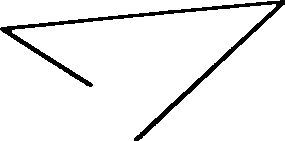
\includegraphics[width=0.75\textwidth]{figures/quad1.png}
	\end{subfigure}
	\begin{subfigure}{0.5\textwidth}
		\centering
		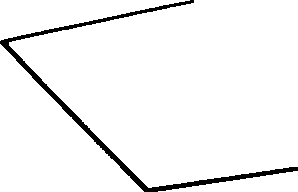
\includegraphics[width=0.75\textwidth]{figures/quad2.png}
	\end{subfigure}
	\caption{Example for different quads}
	\label{fig:exampleQuads}
\end{figure}

%-----------------------------------------------------------------------------------------------
\section{RQIM}
%-----------------------------------------------------------------------------------------------

%-----------------------------------------------------------------------------------------------
\chapter{Marker recognition}\label{sect:markerRec}
%-----------------------------------------------------------------------------------------------

In this chapter there will be a summary of the image processing algorithms tried and used for the recognition of the fiducial markers.
From a computer vision point of view the task is to detect joint line segments.
This is a relatively easy task in image processing, there are many well tried algorithms for it.

In this chapter will be a short summary of the algorithms used for testing and performance comparison.
The preprocessing steps used for preparing the images for the line fitters (segmentation, thresholding, filtering etc.) will also be discussed.

The general flow of processing is the same for every line fitting solution.
The input is the raw image taken\footnote{In the development phase there were rendered pictures used for better repeatability} by the observer.
The first problem is finding the RQIM on the picture.
When the marker area is located, it is necessary to discard the only partially visible and/or unrecognisable quads.
At this point there is an image or set of images containing potentially good quads.
The process here diverges depending on which line fitting algorithm is used.
They all need differently conditioned input images for optimal performance.
The line fitter routines not necessarily have the same output format\footnote{Some return line segments defined by their endpoint, others use the polar representation of a lin, etc.}, so conversion may be needed.
This is the end of the marker recognition phase.
This step of the process takes the raw input image and initiates quad structures based on the observed picture.

Four separate line fitters are profiled in this experiment.
\begin{itemize}
	\item Hough-transformation
	\item Corner detection
	\item Skeletoning detector
	\item Gradient detector (enhanced Hough transformation)
\end{itemize}
The first one uses the classic Hough-transformation for line detection.
In the OpenCV framework there is another, probabilistic implementation of the transformation.
It will also be tested.

The second detector is based on corner recognition.
There are more variants to try out for this method too.
The corner metrics of a feature can be calculated differently with (Harris metric, eigenvalues, etc.) varying results.
It is also needed for the solution to be scale invariant, which also can be achieved in a number of ways.

The third alternative uses skeletoning for line detection.
It is a RANSAC-like method, which makes it very robust, though quite computationally expensive.
The core concept is to thin the observed marker (band) down to single pixel lines and try to find two point with the most inliers.

The gradient detector is a bit Hough-like in it's nature.
It uses the image gradient the calculate the angle in the Hough-space, and the pixels only vote in their distance parameter.

%-----------------------------------------------------------------------------------------------
\section{Preprocessing}
%-----------------------------------------------------------------------------------------------



%-----------------------------------------------------------------------------------------------
\subsection{Segmentation}
%-----------------------------------------------------------------------------------------------



%-----------------------------------------------------------------------------------------------
\subsection{Filtering}
%-----------------------------------------------------------------------------------------------



%-----------------------------------------------------------------------------------------------
\section{Line fitters}
%-----------------------------------------------------------------------------------------------



%-----------------------------------------------------------------------------------------------
\subsection{Hough transformation}
%-----------------------------------------------------------------------------------------------



%-----------------------------------------------------------------------------------------------
\subsection{Gradient detector}
%-----------------------------------------------------------------------------------------------



%-----------------------------------------------------------------------------------------------
\subsection{Corner detector}
%-----------------------------------------------------------------------------------------------



%-----------------------------------------------------------------------------------------------
\subsection{Skeletoning detector}
%-----------------------------------------------------------------------------------------------



%-----------------------------------------------------------------------------------------------
\chapter{Chapter 3}\label{sect:chapter3}
%-----------------------------------------------------------------------------------------------

%-----------------------------------------------------------------------------------------------
\chapter{Conclusion}\label{sect:conclusion}
%-----------------------------------------------------------------------------------------------

During the course of this work the process of calculating camera pose was thoroughly examined.
Each step from getting the input image to calculating the camera pose was discussed.
For most parts both the underlying theory and empirical test results were presented.

In line with the project targets, multiple pose estimation methods were discussed and compared.
The EP$n$P\cite{Lepetit2008}, an iterative approach\cite{iterative} and the robust pose estimation\cite{robust} were considered as candidates to be used in this project.
Short summaries of their operating principles were presented.
Their performance then was compared with respect to multiple properties: accuracy, robustness, and computational efficiency.
As a result, two algorithms were selected depending on the available computational power available on the target platform.
EP$n$P is recommended for use on mobile devices or embedded platforms, where efficient, non-iterative solution is preferred.
However, if robust and accurate results are necessary (and there are enough resources), the robust pose estimation algorithm is the better choice.

Another focus of the project was developing a marker with advantageous properties for pose estimation.
To achieve this goal the RQIM was proposed.
It is a randomly generated marker put together from multiple quads.
It has been shown to have desirable properties for pose estimation: scale invariance and redundancy.
A formal representation of the quads (both mathematical and computational) have been defined.
A simple algorithm was proposed for generating random markers.
The notion of creating discrete parameter space for quads has also been examined.
It would provide additional robustness and the ability to encode meta-information in the markers, however these possibilities have not been tested.

The main part of this work is dedicated to the development and testing of a marker detecting solution.
It was shown that marker detection is (from an image processing point of view) equivalent to detecting individual quads on the source image.
Two different approaches were made to quad detection: line detection-, and corner detection based solution.
Multiple line detection algorithms were considered for use.
To make a more informed decision on which one to use, their theoretical foundations have been summarised.
The theory of corner detection was also covered.
Four different quad detectors were developed and tested: each based on a different underlying algorithm.
Their implementation details were discussed and their python source code is published in the appendix.

The quad detectors were not only compared based on the theoretical capabilities of their underlying algorithm, they were also extensively tested.
A testing methodology have been developed for comparing the algorithms.
The test were run on randomly generated quads with fixed sizes.
For each size, a 1000 instance was generated to guarantee that the results are statistically significant.
To quantify the detection error, multiple error functions were defined.
The detectors were compared by the ones that describe the overall error in detection.
Error functions were defined for each quad parameter; with their help, the distribution of inaccuracy between the parameters were examined.

Based on the data obtained by the tests, the LSD\cite{LSDDet} line detector based implementation was selected.
It proved to be the most accurate and resistant to noise.
It is also an efficient algorithm that runs in linear time.

The final part of this work was about organising the above components into a complete pose estimation solution.
Images used as input for pose estimation have to be preprocessed and filtered for noise.
These steps of the processing pipeline have been described in chapter 4.
The detected quad structures of a marker are used as input for the pose estimation algorithms selected in chapter 1.
A RANSAC-like approach was proposed for finding the correspondences between the detected and the original quads.
%\listoffigures\addcontentsline{toc}{chapter}{Ábrák jegyzéke}
%\listoftables\addcontentsline{toc}{chapter}{Táblázatok jegyzéke}

\bibliography{mybib}
\addcontentsline{toc}{chapter}{Bibliography}
\bibliographystyle{plain}

%----------------------------------------------------------------------------
\appendix
%----------------------------------------------------------------------------
\chapter*{Appendix}\addcontentsline{toc}{chapter}{Appendix}
\setcounter{chapter}{1}  % a fofejezet-szamlalo az angol ABC 6. betuje (F) lesz
\setcounter{equation}{0} % a fofejezet-szamlalo az angol ABC 6. betuje (F) lesz
\numberwithin{equation}{section}
\numberwithin{figure}{section}
\numberwithin{lstlisting}{section}
%\numberwithin{tabular}{section}


\label{page:last}
\end{document}